\documentclass{article}
\usepackage{enumitem}
\usepackage{array}
\usepackage{subcaption}
\usepackage{graphicx}
\usepackage{subcaption}

\usepackage{color}
\usepackage[top=1in,bottom=1in,left=1.2in,right=1.2in]{geometry}
\usepackage{hyperref}
\usepackage[small]{titlesec}
\usepackage{booktabs}
\usepackage{colm2024_conference}
\usepackage{graphicx}
\usepackage[dvipsnames]{xcolor}
\usepackage{rotating}
\usepackage{pdflscape}
\usepackage{amsmath}

\newcommand{\todo}[1]{\textcolor{red}{\textbf{TODO:} #1}}

% Commenting
\newcommand{\eat}[1]{\ignorespaces}
%% Comment this line and uncomment the next to hide all comments
\newcommand{\xxcomment}[4]{\textcolor{#1}{[$^{\textsc{#2}}_{\textsc{#3}}$ #4]}}
\newcommand{\ta}[1]{\xxcomment{blue}{T}{A}{#1}}


\title{CS5787: Exercises 3 \\ \begin{small}\url{https://github.com/mitkrieg/dl-assignment-3}\end{small}}
\author{Mitchell Krieger \\ mak483@cornell.edu}

\date{}

\colmfinalcopy
\begin{document}
\maketitle

\section{Theory: Question 1 [40 pts]}

\begin{enumerate}[label=\alph*)]
    \item $\theta \neq 0$
        \begin{itemize}
            \item KL Divergence: \\ When $\theta = 0$ there is no overlap between P and Q. This means that whenever P is greater than zero, Q is zero. Applying this to the 
            KL formula at $x=0$ and assume that we can represent x as the Dirac delta function $\delta(x)$, and $u(y)$ is the uniform distribution over [0,1].
            \begin{equation}
                \begin{aligned}
                    D_{KL}(P||Q) &= \int_{x=-\infty}^{\infty} \int_{y=-\infty}^{\infty} P(x,y)\log \frac{P(x,y)}{Q(x,y)}dydx
                    \\ &= \int_{x=-\infty}^{\infty} \int_{y=-\infty}^{\infty} \delta(x)\cdot u(y)\log \frac{\delta(x)\cdot u(y)}{\delta(x-\theta)\cdot u(y)}dydx
                    \\ &= \int_{x=-\infty}^{\infty} \delta(x)  \int_{y=0}^{1} \log(\frac{\delta(x)\cdot 1}{\delta(x-\theta)\cdot 1}) dx
                \end{aligned}
            \end{equation}
            Since, $\delta(x)$ is zero everywhere except $x=0$
            \begin{equation}
                \begin{aligned}
                    D_{KL}(P||Q) &= \int_{y=0}^{1} \log(\frac{\delta(0)}{\delta(-\theta)}) dy
                    \\ &=  \frac{\delta(0)}{0} = \infty
                \end{aligned}
            \end{equation}
            We can see from the above that because the logarithm in the equation is undefined, we get a value for KL Divergence that tends to $\infty$.\\
            \item JS Divergence: \\ The JS Divergence considers the KL Divergence between each distribution and the average of the two distributions.
            The average distribution $\frac{P+Q}{2}$ will split the distribution to be half at $x = 0$ and half at $x = \theta$. Therefore, The KL Divergence between
            P and the average will be:
            \begin{equation}
                \begin{aligned}
                    D_{KL}(P||\frac{P+Q}{2}) &= \int_{x=-\infty}^{\infty} \int_{y=-\infty}^{\infty} P(x,y)\log \frac{P(x,y)}{\frac{1}{2}P(x,y)+\frac{1}{2}Q(x,y)}dydx
                    \\ &= \int_{x=-\infty}^{\infty} \delta(x)  \int_{y=0}^{1} \log(\frac{\delta(x)\cdot u(y)}{\frac{1}{2}\delta(x)\cdot u(y)+\frac{1}{2}\delta(x-\theta)\cdot u(y)})
                \end{aligned}
            \end{equation}
            Since, $\delta(x)$ is zero everywhere except $x=0$, and $\delta(x-\theta) = 0$ at $x=0$
            \begin{equation}
                \begin{aligned}
                    D_{KL}(P||\frac{P+Q}{2}) &= \int_{y=0}^{1} \log(\frac{\delta(0))\cdot u(y)}{\frac{1}{2}\delta(0)\cdot u(y)+\frac{1}{2}\cdot0\cdot u(y)})
                    \\  &=  \log(\frac{1}{\frac{1}{2}}) 
                    \\  &= \log(2)
                \end{aligned}
            \end{equation}

            $D_{KL}(Q||\frac{P+Q}{2})$ will give the same result. So applying the JS Divergence formula:
            \begin{equation}
                \begin{aligned}
                    D_{JS}(P||Q) = \frac{1}{2} \cdot \log(2) + \frac{1}{2} \cdot \log(2) = \log(2)
                \end{aligned}
            \end{equation}
            \\
            \item Wasserstein Distance: \\ The Wasserstein Distance is $\theta$ because both distributions have the same uniform distribution between [0,1] for $y$. 
            Because they are identical except for the x-value of P is 0 and the x-value of Q is $\theta$, the cost of moving P to Q would be $\theta$.
        \end{itemize}  
    \item $\theta = 0$
        \begin{itemize}
            \item KL Divergence: \\ Zero because the distributions are the same
            \begin{equation}
                \begin{aligned}
                    D_{KL}(P||Q) &= \int_{-\infty}^{\infty} \int_{-\infty}^{\infty} P(x)\log \frac{P(x,y)}{P(x,y)}dydx\\
                    &= \int_{-\infty}^{\infty} \int_{-\infty}^{\infty} P(x,y)\log1 dydx\\
                    &= \int_{-\infty}^{\infty} \int_{-\infty}^{\infty} 0\cdot P(x,y)  dydx\\
                    &= 0
                \end{aligned}
            \end{equation}
            \item JS Divergence: \\ $\frac{P+Q}{2} = P = Q$ because both distributions are uniform between [0,1] for $y$ and centered at $x = 0$. So the JS Divergence is zero because the distributions are the same
            \begin{equation}
                \begin{aligned}
                    D_{JS}(P||Q) &= \frac{1}{2}D_{KL}(P||\frac{P+Q}{2}) + \frac{1}{2}D_{KL}(Q||\frac{P+Q}{2}) \\
                                 &= \frac{1}{2} \cdot 0 + \frac{1}{2} \cdot 0 = 0
                \end{aligned}
            \end{equation}
            \item Wasserstein Distance: Zero because both distributions are uniform between [0,1] for $y$ and centered at $x = 0$. So there is no cost to transform P into Q.
    
    \end{itemize}  
    \item The advantage of the Wasserstein Distance is that it is both interpretable and stable when compared to KL and JS Divergence. When $\theta \neq 0$,
    KL is infinite and JS is $\log2$, where as Wasserstein is $\theta$. In this context, $\theta$ is a much clearer measure of the distances between the two 
    distribution because it is simply the distance between the x-values of the distributions. In addition, both KL and JS have discontinuous jumps from when 
    they overlap to when then don't, KL becomes infinite and JS although still finite jumps from 0 to $\log2$. Wasserstein distance on the other hand, increases linearly as 
    $\theta$ grows. These are big advantages because it would make the gradient in training a model more stable because it is continuous and not super sensitive to small changes (from not overlapping to overlapping).

\end{enumerate}


\section{Theory: Question 2 [10 pts]}

LSTMs will process inputs sequentially. So at each time step, the LSTM will have to multiply the input by the hidden state, the previous hidden state by the current hidden state,
and other smaller operations like the activation functions for the gates and addition for adding bias and cell state updates. The dominant operation here is the multiplication of the 
hidden states. This operation has a time complexity of $O(d^2)$ where $d$ is the dimension of the hidden state. Because we do this at every time step t for all $N$, the total complexity is $O(d^2N)$.
However, the size of the hidden state is a constant value, and not a function of the size of the input, so the total time complexity is linear $O(N)$.

Transformers on the other hand use self-attention, which requires every value of the input to be compared to all other values in the input. This is an $O(N^2)$ operation. The other components
of transformers, such as the feed forward network, encoder/decoder and positional encoding are all generally $O(N)$, so they get dominated by the self-attention mechanism's computational complexity.
So the total time complexity is quadratic at $O(N^2)$

\section{Practical: Question 3 [5 pts]}

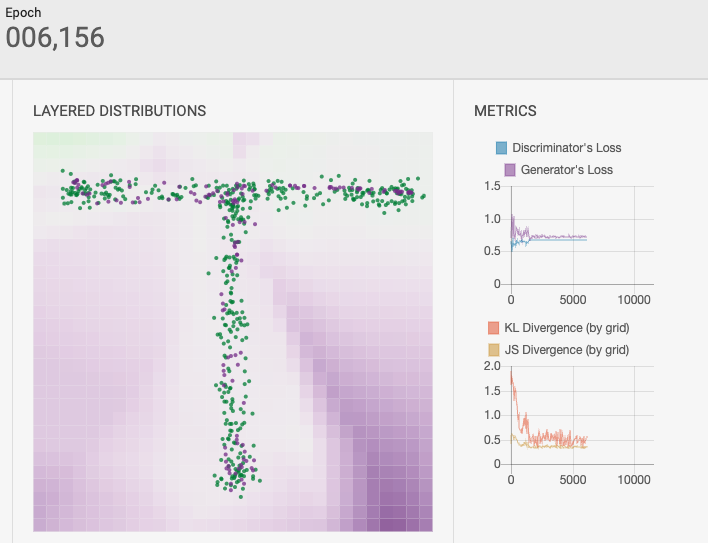
\includegraphics[scale=.5]{../src/gan_lab.png}

\section{Practical: Question 4 [20 pts]}

\section{Practical: Question 5 [25 pts]}

\end{document}